\documentclass[a4paper,11pt]{article}
\usepackage{graphicx}
\usepackage[]{latexsym}
\usepackage[]{amsmath}
\usepackage[]{mathtools}
\usepackage[]{bm}
\usepackage[MeX]{polski}
\usepackage[utf8]{inputenc}

\author{Wojciech Lepich \and Nomen Nescio}
\title{NUM5. Metody iteracyjne Jacobiego i \nolinebreak{Gaussa-Seidela}}

\begin{document}
\maketitle
\section{Teoria}
Metody iteracyjne służą do znalezienia rozwiązania układu równań z pewnym przybliżeniem.
Teoretycznie w granicy nieskończenie wielu kroków otrzymujemy dokładne rozwiązanie.
Dwie z metod to metoda Jacobiego i metoda Gaussa-Seidela.

\subsection{Metoda Jacobiego}
Rozwiązaniem układu \(Ax = B\) z daną macierzą \(A\) i wektorem \(b\) jest:
\[ x_{i}^{(k+1)} = \frac{1}{a_{ii}}(b_{i} - \sum_{j=1}^{i-1}a_{ij}x_{j}^{(k)} 
- \sum_{j=i+1}^{N}a_{ij}x_{j}^{(k)}) \]
Metoda Jacobiego jest zbieżna, jeśli macierz A jest silnie diagonalnie dominująca.

\subsection{Metoda Gaussa-Seidela}
Rozwiązaniem układu \(Ax = B\) z daną macierzą \(A\) i wektorem \(b\) jest:
\[ x_{i}^{(k+1)} = \frac{1}{a_{ii}}(b_{i}-\sum_{j=1}^{i-1}a_{ij}x_{j}^{(k+1)} - 
\sum_{j=i+1}^{N}a_{ij}x_{j}^{(k)}) \]
W tej metodzie obliczając \(x_{i}^{(k+1)}\)-ty element korzystamy z najnowszych przybliżeń 
\(x_{j}^{(k+1)}\) dla \(j<i\). W omówieniu widać korzyści płynące z tego ulepszenia. Wadą 
rozwiązania jest niemożność zrównoleglenia obliczeń.

\section{Omówienie}
Zadany jest układ równań
\[
    \left(
        \begin{matrix}
            3 & 1 & 0.2 & & & & & \\
            1 & 3 & 1 & 0.2 & & & & \\
            0.2 & 1 & 3 & 1 & 0.2 & & & \\
            \cdots & \cdots & \cdots & \cdots & \cdots & \cdots & \\
            & & & 0.2 & 1 & 3 & 1 \\
            & & & & 0.2 & 1 & 3
        \end{matrix}
    \right)  
    \bm{\text{\bf{x}}} = 
    \left(
        \begin{matrix}
            1 \\ 2 \\ 3 \\ \cdots \\ N-1 \\ N
        \end{matrix}
    \right)
\]
Po lewej stronie równania jest macierz diagonalna, silnie diagonalnie dominująca o wymiarze N.
Przy tej strukturze macierzy \(x_{i}\), dla \(i \in [3;N-2]\) będzie dany równaniem
\[
    x_{i} = \frac{1}{a_{ii}}(b_{i} - a_{i,i-2}x_{i-2} - a_{i,i-1}x_{i-1} 
    - a_{i,i+1}x_{i+1}-a_{i,i+2}x_{i+2})
\]
Przy każdym obliczaniu \(x_{i}\) redukujemy ilość dodawań z \(N-1\) na \(4\).
Dla \(i = 1, 2, N, N-1\) ze wzoru pozbywamy się wyrazu, 
którego otrzymanie byłoby próbą wydostania się poza wymiary macierzy 
--- na przykład dla \(i = 1\) pozbywamy się wyrazów \(a_{i, i-2}x_{i-2}\) oraz 
\(a_{i, i-1}x_{i-1}\).

\subsection{Różnice w implementacji metod}
W obydwu metodach iteracja przebiega następująco:
\begin{enumerate}
    \item Obliczenie wyrazów \(x_{1}\) i \(x_{2}\)
    \item Obliczenie w pętli wyrazów od \(x_{3}\) do \(x_{N-2}\)
    \item Obliczenie wyrazów \(x_{N-1}\) i \(x_{N}\)
\end{enumerate}

W metodzie Jacobiego kolejność kroków może być zamieniona.

Różnice pojawiają się w przechowywaniu nowych wartości. W obydwu przypadkach potrzebujemy dwóch 
tablic --- jedną na nowo obliczone wartości, drugą na wartości z poprzedniej iteracji.
W metodzie Jacobiego po znalezieniu kolejnej iteracji \(\bm{\text{\bf{x}}}\) i sprawdzeniu czy 
otrzymaliśmy wynik przypisujemy te wartości do ,,starej'' tablicy (tej, z której bierzemy 
wartości do obliczania wyrazów \(\bm{\text{\bf{x}}})\) i idziemy do kolejnej iteracji.

W metodzie Gaussa-Seidela nowe wartości wstawiamy do tej samej tablicy, z której odczytujemy do 
obliczania wyrazów \(\bm{\text{\bf{x}}}\). Druga tablica jest nam potrzebna, aby sprawdzić czy
zbliżyliśmy się wystarczająco do rozwiązania --- wartości do niej kopiujemy na początku pętli.

\pagebreak
Na wykresie widać szybkość zbiegania kolejnych przybliżeń \(\bm{\text{\bf{x}}}\) w \(i\)-tej 
iteracji do właściwego rozwiązania. Metoda Gaussa-Seidela po 29 iteracjach dała rozwiązanie
identyczne z wynikiem otrzymanym w Mathematice. Metoda Jacobiego zbiegała dużo wolniej i dopiero
po 155 iteracji otrzymano rozwiązanie.

% GNUPLOT: LaTeX picture with Postscript
\begingroup
  \makeatletter
  \providecommand\color[2][]{%
    \GenericError{(gnuplot) \space\space\space\@spaces}{%
      Package color not loaded in conjunction with
      terminal option `colourtext'%
    }{See the gnuplot documentation for explanation.%
    }{Either use 'blacktext' in gnuplot or load the package
      color.sty in LaTeX.}%
    \renewcommand\color[2][]{}%
  }%
  \providecommand\includegraphics[2][]{%
    \GenericError{(gnuplot) \space\space\space\@spaces}{%
      Package graphicx or graphics not loaded%
    }{See the gnuplot documentation for explanation.%
    }{The gnuplot epslatex terminal needs graphicx.sty or graphics.sty.}%
    \renewcommand\includegraphics[2][]{}%
  }%
  \providecommand\rotatebox[2]{#2}%
  \@ifundefined{ifGPcolor}{%
    \newif\ifGPcolor
    \GPcolortrue
  }{}%
  \@ifundefined{ifGPblacktext}{%
    \newif\ifGPblacktext
    \GPblacktexttrue
  }{}%
  % define a \g@addto@macro without @ in the name:
  \let\gplgaddtomacro\g@addto@macro
  % define empty templates for all commands taking text:
  \gdef\gplbacktext{}%
  \gdef\gplfronttext{}%
  \makeatother
  \ifGPblacktext
    % no textcolor at all
    \def\colorrgb#1{}%
    \def\colorgray#1{}%
  \else
    % gray or color?
    \ifGPcolor
      \def\colorrgb#1{\color[rgb]{#1}}%
      \def\colorgray#1{\color[gray]{#1}}%
      \expandafter\def\csname LTw\endcsname{\color{white}}%
      \expandafter\def\csname LTb\endcsname{\color{black}}%
      \expandafter\def\csname LTa\endcsname{\color{black}}%
      \expandafter\def\csname LT0\endcsname{\color[rgb]{1,0,0}}%
      \expandafter\def\csname LT1\endcsname{\color[rgb]{0,1,0}}%
      \expandafter\def\csname LT2\endcsname{\color[rgb]{0,0,1}}%
      \expandafter\def\csname LT3\endcsname{\color[rgb]{1,0,1}}%
      \expandafter\def\csname LT4\endcsname{\color[rgb]{0,1,1}}%
      \expandafter\def\csname LT5\endcsname{\color[rgb]{1,1,0}}%
      \expandafter\def\csname LT6\endcsname{\color[rgb]{0,0,0}}%
      \expandafter\def\csname LT7\endcsname{\color[rgb]{1,0.3,0}}%
      \expandafter\def\csname LT8\endcsname{\color[rgb]{0.5,0.5,0.5}}%
    \else
      % gray
      \def\colorrgb#1{\color{black}}%
      \def\colorgray#1{\color[gray]{#1}}%
      \expandafter\def\csname LTw\endcsname{\color{white}}%
      \expandafter\def\csname LTb\endcsname{\color{black}}%
      \expandafter\def\csname LTa\endcsname{\color{black}}%
      \expandafter\def\csname LT0\endcsname{\color{black}}%
      \expandafter\def\csname LT1\endcsname{\color{black}}%
      \expandafter\def\csname LT2\endcsname{\color{black}}%
      \expandafter\def\csname LT3\endcsname{\color{black}}%
      \expandafter\def\csname LT4\endcsname{\color{black}}%
      \expandafter\def\csname LT5\endcsname{\color{black}}%
      \expandafter\def\csname LT6\endcsname{\color{black}}%
      \expandafter\def\csname LT7\endcsname{\color{black}}%
      \expandafter\def\csname LT8\endcsname{\color{black}}%
    \fi
  \fi
    \setlength{\unitlength}{0.0500bp}%
    \ifx\gptboxheight\undefined%
      \newlength{\gptboxheight}%
      \newlength{\gptboxwidth}%
      \newsavebox{\gptboxtext}%
    \fi%
    \setlength{\fboxrule}{0.5pt}%
    \setlength{\fboxsep}{1pt}%
\begin{picture}(7200.00,5040.00)%
    \gplgaddtomacro\gplbacktext{%
      \csname LTb\endcsname%%
      \put(814,704){\makebox(0,0)[r]{\strut{}$-14$}}%
      \put(814,1163){\makebox(0,0)[r]{\strut{}$-12$}}%
      \put(814,1623){\makebox(0,0)[r]{\strut{}$-10$}}%
      \put(814,2082){\makebox(0,0)[r]{\strut{}$-8$}}%
      \put(814,2542){\makebox(0,0)[r]{\strut{}$-6$}}%
      \put(814,3001){\makebox(0,0)[r]{\strut{}$-4$}}%
      \put(814,3460){\makebox(0,0)[r]{\strut{}$-2$}}%
      \put(814,3920){\makebox(0,0)[r]{\strut{}$0$}}%
      \put(814,4379){\makebox(0,0)[r]{\strut{}$2$}}%
      \put(946,484){\makebox(0,0){\strut{}$0$}}%
      \put(1678,484){\makebox(0,0){\strut{}$20$}}%
      \put(2410,484){\makebox(0,0){\strut{}$40$}}%
      \put(3142,484){\makebox(0,0){\strut{}$60$}}%
      \put(3875,484){\makebox(0,0){\strut{}$80$}}%
      \put(4607,484){\makebox(0,0){\strut{}$100$}}%
      \put(5339,484){\makebox(0,0){\strut{}$120$}}%
      \put(6071,484){\makebox(0,0){\strut{}$140$}}%
      \put(6803,484){\makebox(0,0){\strut{}$160$}}%
    }%
    \gplgaddtomacro\gplfronttext{%
      \csname LTb\endcsname%%
      \put(209,2541){\rotatebox{-270}{\makebox(0,0){\strut{}$\log10|x^{(i)}-x^{*}|$}}}%
      \put(3874,154){\makebox(0,0){\strut{}i}}%
      \put(3874,4709){\makebox(0,0){\strut{}Przyblizenia}}%
      \csname LTb\endcsname%%
      \put(5816,4206){\makebox(0,0)[r]{\strut{}Gauss-Seidel}}%
      \csname LTb\endcsname%%
      \put(5816,3986){\makebox(0,0)[r]{\strut{}Jacobi}}%
    }%
    \gplbacktext
    \put(0,0){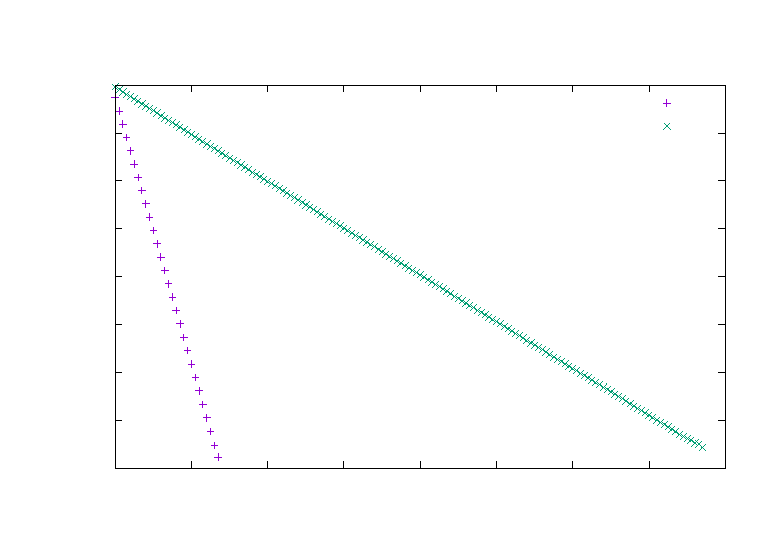
\includegraphics{plot}}%
    \gplfronttext
  \end{picture}%
\endgroup

\end{document}
